\newpage
\chapter{Mode Decomposition}
\label{ch:ch2}

\section{Vertical and Horizontal Structure Equations}
The main goal of decomposing the energy spectra into geostrophic and ageostrophic motion is to separate the fast gravity waves from the slow balanced vortices. To that end, consider linearizing the governing equations (\ref{eq:momentumFull} -\ref{eq:thermodynamicFull}) about a state of rest, as commonly done in the literature (e.g.\ \cite{Daley1991}, \cite{Kasahara1981}). While a more complicated basic state can be used (e.g.\ a non-zero zonal mean flow), the primary interest is of the inertia gravity wave modes that are initialized by the baroclinic instabilities. These gravity wave modes have  much shorter characteristic timescales than the slowly rotating geostrophic part and are not strongly influenced by a linearization about a more realistic basic state involving the zonal mean velocity field, e.g.\ \cite{Dickinson1972}. The equations of motion linearized about a state of rest with a basic state geopotential $\tilde{\Phi}$ then result in the following system of equations

\begin{align}
&\frac{\partial u'} {\partial t} - fv' = -\frac{\partial \Phi'}{\partial x},\label{eq:nmMomentum}\\
&\frac{\partial v'} {\partial t} + fu' = -\frac{\partial \Phi'}{\partial y},\\
&\nabla \cdot \mathbf{u'} + \frac{\partial \omega}{\partial p} = 0,\label{eq:nmCont}\\
&\frac{\partial}{\partial t} \frac{\partial \tilde{\Phi}}{\partial p} + \omega \tilde{\Gamma} \label{eq:nmThermo} = 0.
\end{align}

For the rest of this section, the prime notation seen on $u$, $v$, and $\Phi$ to represent the deviation from the basic state is omitted except for where confusion would occur otherwise. Following the approach of Daley \cite{Daley1991}, equations (\ref{eq:nmCont}) and (\ref{eq:nmThermo}) can be combined to reduce the system of equations to three equations and three unknowns shown below:

\begin{align}
&\frac{\partial u} {\partial t} - fv = -\frac{\partial \Phi}{\partial x},\label{eq:nmLinMom}\\
&\frac{\partial v} {\partial t} + fu = -\frac{\partial \Phi}{\partial y},\\
&\frac{\partial}{\partial p} \left( \frac{1}{\tilde{\Gamma}} \frac{\partial }{\partial t} \frac{\partial \tilde{\Phi}}{\partial p}\right) - \nabla \cdot \mathbf{u} = 0. \label{eq:nmThermoHydro}
\end{align}

Since (\ref{eq:nmThermoHydro}) contains all of the explicit vertical derivatives, it is appropriate to separate the vertical dependence of the velocity and geopotential fields from the horizontal dependence, i.e.\ let 
\begin{align}
&u(x,y,p,t) = U(x,y,t) Z(p),\label{eq:separationBegin}\\
&v(x,y,p,t) = V(x,y,t) Z(p),\\
&\Phi(x,y,p,t) = \Phi^*(x,y,t) Z(p).\label{eq:separationEnd}
\end{align}
Substituting this separation into equations (\ref{eq:nmLinMom} - \ref{eq:nmThermoHydro}) gives
\begin{align}
&\frac{\partial U}{\partial t} - fV = -\frac{\partial \Phi^*}{\partial x},\\
&\frac{\partial V}{\partial t} + fU = -\frac{\partial \Phi^*}{\partial y},\\
&\frac{1}{Z}\frac{\text{d}}{\text{d} p} \left(\frac{1}{\tilde{\Gamma}}\frac{\text{d} Z}{\text{d} p}\right) = \frac{1}{\frac{\partial \Phi^*}{\partial t}} \left(\frac{\partial U}{\partial x} + \frac{\partial V}{\partial y}\right) = -\frac{1}{gh_n}, \label{eq:separation}
\end{align}
where $-1/gh$ is a separation constant chosen to be dimensionally consistent with the left-hand side and middle of equation (\ref{eq:separation}). The equations of motion are now in a separated state consisting of horizontal structure

\begin{align}
&\frac{\partial U}{\partial t} - fV = -\frac{\partial \Phi^*}{\partial x}, \label{eq:nmHorizBegin}\\
&\frac{\partial V}{\partial t} + fU = -\frac{\partial \Phi^*}{\partial y},\\
&\left(\frac{\partial U}{\partial x} + \frac{\partial V}{\partial y}\right) + \frac{1}{gh_n} \frac{\partial \Phi^*}{\partial t} = 0, \label{eq:nmHorizEnd}
\end{align}
and vertical structure
\begin{align}
\frac{\text{d}}{\text{d} p} \left( \frac{1}{\tilde{\Gamma}}\frac{\text{d} Z}{\text{d} p} \right) + \frac{1}{gh_n} Z = 0, \label{eq:nmVert}
\end{align}
coupled together by the $1/gh_n$ term. This coupling is only valid if the divergence is non-zero. Note that the horizontal eigenvalue problem is valid only for an $f$-plane approximation and that a $\beta$-plane approximation would result in a different eigenvalue problem in the horizontal. Later in this chapter, the case of geostrophic motion is dealt with. Bearing this in mind, we now focus our attention solely on the vertical structure problem (\ref{eq:nmVert}) of a flow with non-zero divergence, returning to the horizontal problem in Section \ref{sec:horiz} and geostrophic motion in Section \ref{sec:geostrophicMotion} .

\section{Vertical Normal Modes}
\subsection{A Brief Outline of Sturm-Liouville Theory}
A Sturm-Liouville (S-L) problem is a type of ordinary differential equation (ODE) of the form
\begin{align}
\frac{\text{d}}{\text{d} p} \left( s(p) \frac{\text{d} Z}{\text{d} p} \right) + q(p) Z + \lambda w(p) Z = 0, \label{eq:SturmLiouville}
\end{align}
with non-zero $s(p)$ and $w(p)$. Here, $s(p)$, $q(p)$, and $w(p)$ are given functions, with $w(p)$ being the ``weighting'' function. This is an eigenvalue problem, with eigenvalue $\lambda$. There are many nice properties of solutions of S-L problems. We are interested in the orthogonality of eigenfunctions with respect to the weighting $w(p)$ and the guarantee of real, non-degenerate eigenvalues. That is, the eigenvalues can be arranged in an increasing order, and the inner product with respect to $w$ gives an orthonormality condition 
\begin{align}
(f_j, f_k)_w = \int_a^b \overline{f_j(p)}f_k(p) w(p) ~\text{d}p = \delta_{jk} \label{eq:orthonormamiltyHard}
\end{align}
for normalized eigenfunctions $f_j(p)$, $f_k(p)$ and appropriate boundary conditions at $p=a,b$. In addition to the orthogonality, eigenfunctions of a S-L problem are complete. Refer to any ODE text for a review (e.g. \cite{Atkinson1964}).\\

From this, it is clear that the vertical structure equation (\ref{eq:nmVert}) is a S-L ODE with $q(p) = 0$ and $s(p) = 1/\tilde{\Gamma}(p)$, $\lambda = 1/gh$, and $w(p) = 1$. The orthogonality condition (\ref{eq:orthonormamiltyHard}) simply becomes an inner product given by

\begin{align}
(f_j, f_k) = \frac{1}{p_s} \int_0^{p_s} \overline{f_j(p)} f_k(p) ~\text{d}p = \delta_{jk},
\end{align}
where $p_s$ is the pressure at the surface. The $n^{th}$ eigenvalue in the vertical structure problem (\ref{eq:nmVert}) is $1/gh_n$, where the subscript $n$ is added to $h$ to represent what can be thought of as a ``equivalent depth'' \cite{Daley1991} of the $n^{th}$ vertical mode.\\

\subsection{Numerical Solution and Boundary Conditions}
\label{sec:normalModes}
In order for the problem to be well-posed, two boundary conditions are needed for the second-order differential equation. The boundary conditions for (\ref{eq:nmVert}) are now derived, following \cite{Daley1991}.\\

At the bottom, the assumption is a flat ground with no topography, and so the appropriate choice is 
\begin{align}
\frac{\text{D} \Phi}{\text{D} t}  = \frac{\partial \Phi'}{\partial t} + \mathbf{u} \cdot \nabla \Phi + \omega \frac{\partial}{\partial p} (\tilde{\Phi} + \Phi') = 0,
\end{align}
where the geopotential is decomposed into a basic state, $\tilde{\Phi}(p)$, and a variation from this basic state $\Phi'(x,y,t)$ such that $\Phi = \tilde{\Phi} + \Phi'$. Also, we use the notation $\mathbf{u} = (u,v)$ and $\omega = dP/dt$ is the vertical velocity in pressure coordinates. Dropping the non-linear terms results in
\begin{align}
\frac{\partial \Phi'}{\partial t} + \omega \frac{\partial \tilde{\Phi}}{\partial p} = 0.\\
\end{align}
Using the hydrostatic equation (\ref{eq:hydrostatic}) to eliminate $\partial \tilde{\Phi}/\partial p$ results in
\begin{align}
\frac{\partial \Phi}{\partial t}  - \omega \frac{R\tilde{T}}{p} = 0,
\end{align}
and using the thermodynamic equation (\ref{eq:nmThermo}) eliminate $\omega$ gives
\begin{align}
\frac{\partial \Phi}{\partial t}  + \left(\frac{1}{\tilde{\Gamma}} \frac{\partial}{\partial t} \frac{\partial \Phi}{\partial p}\right) \frac{R\tilde{T}}{p} = 0.
\end{align}
Finally, substituting the separation of horizontal and vertical dependence (\ref{eq:separationBegin} - \ref{eq:separationEnd}), the bottom boundary condition is 

\begin{align}
\frac{\text{d}Z}{\text{d}p} + \frac{p_s\tilde{\Gamma}}{RT_s} Z = 0 ~~~~\text{at}~ p = p_s,\label{eq:BCbot}
\end{align}
where $p_s$ and $T_s$ refer to the surface pressure and temperature, respectively.\\

The top boundary condition is similarly derived by assuming a rigid lid approximation. This leads to 
\begin{align}
\frac{\text{d}Z}{\text{d}p} + \frac{p_t\tilde{\Gamma}}{RT_t} Z = 0,
\end{align}
where $p_t$ and $T_t$ refer to the pressure and temperature at the top, respectively. Allowing $p \to 0$ to approximate the top of the atmosphere, the top boundary condition is
\begin{align}
\frac{\text{d}Z}{\text{d}p} = 0 ~~~~\text{as}~ p \to 0.\label{eq:BCtop}
\end{align}

Together, equations (\ref{eq:nmVert}), (\ref{eq:BCtop}), and (\ref{eq:BCbot}) completely define the vertical eigenvalue problem.\\

This eigenvalue problem is solved numerically on 100 evenly spaced grid levels using a second order centered finite difference scheme. To handle the boundary condition at $p = 0$, where $\tilde{\Gamma} \to \infty$, a staggered grid approach is taken (e.g. \cite{Kasahara1981}) with $K$ levels. The problem given by equation (\ref{eq:nmVert}) is discretized as follows

\begin{align}
\frac{1}{0.5(\Delta p_i + \Delta p_{i+1})} \left[\frac{1}{\tilde{\Gamma}_{i+1/2}} \left(\frac{\text{d} Z}{\text{d} p}\right)_{i+1/2}  - ~\frac{1}{\tilde{\Gamma}_{i-1/2}} \left(\frac{\text{d} Z}{\text{d} p}\right)_{i-1/2} \right] + \frac{1}{gh_n} Z_i = 0,
\end{align}
where $i+1/2$ is the pressure level in between the $i^{th}$ and $(i+1)^{th}$ grid level and $\Delta p_i$ is the pressure difference between the $i^{th}$ and $(i+1)^{th}$ level. This leads to
\begin{align}
\frac{1}{0.5(\Delta p_i + \Delta p_{i+1})} \left[\frac{1}{\tilde{\Gamma}_{i+1/2}} \frac{Z_{i+1} - Z{i}}{\Delta p_{i+1}}  - ~\frac{1}{\tilde{\Gamma}_{i-1/2}} \frac{Z_i - Z_{i-1}}{\Delta p_i} \right] + \frac{1}{gh_n} Z_i = 0.
\end{align}

The boundary condition at the surface is implemented by using a ghost point, $Z_{K+1}$,

\begin{align}
\frac{Z_{K+1} - Z_K}{\Delta p_{K+1}} = -\frac{p_s \tilde{\Gamma}_s}{RT_s} \frac{(Z_{K+1} + Z_K)}{2},
\end{align}

which can be eliminated by expressing in terms of $Z_k$. An example of the first three modes computed for $\tilde{\Gamma}(p)$ taken from our simulation discussed in Chapter \ref{ch:ch3} are shown in Figure \ref{fig:normalmodes}.

\begin{figure}[H]
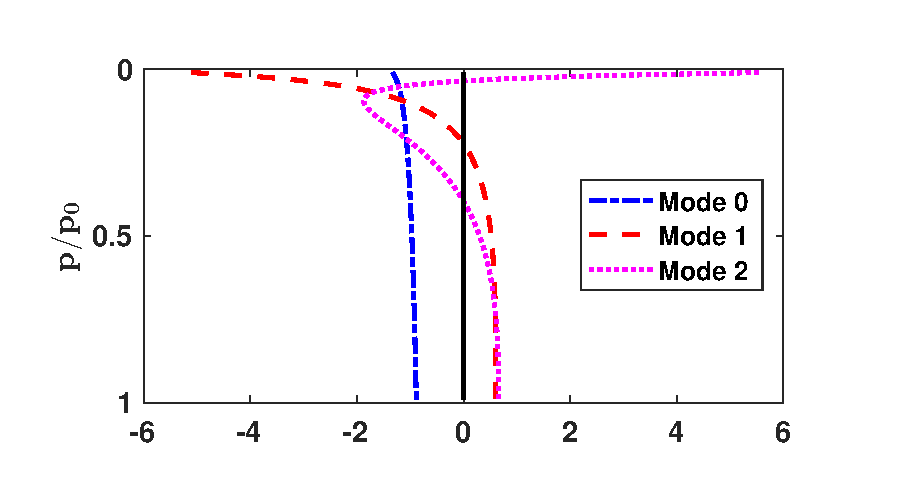
\includegraphics[scale=1]{./Chapter2/img/normalmodes}
\caption{The first three normal modes computed numerically. The equivalent depths are $h_0 = 9400$ m, $h_1 = 1270$ m, and $h_3 = 464$ m. The basic state $\tilde{\Gamma}(p)$ is given by equation (\ref{eq:staticstability}).}
\label{fig:normalmodes}
\end{figure}

The vertical modes are well resolved for most of the first 20. Beyond that, issues with under-resolving the modes start to appear. However, the issues resolving the modes appears to be located near the upper boundary, where the flow velocities are small (see Chapter \ref{ch:ch3}). Additionally, most of the energy is contained in the first several vertical modes (see Figures \ref{fig:modal_energy} and \ref{fig:modal_energy_nobaro}). The numerically computed modes still satisfy the orthonormality condition, and so energy from the more energetic modes do not contaminate the higher modes. Table \ref{tab:equivDepths} shows the computed equivalent depths for the first 30 vertical modes as well as the ratio $f/c_n$ (both dimensional and dimensionless), where $c_n = \sqrt{gh_n}$, which will be further discussed in Chapters \ref{ch:ch4} and \ref{ch:ch5}. For conciseness, only the odd numbered modes are shown. \\

\begin{table}
\begin{center}
\begin{tabular}{c c c c}

\hline
Vertical Mode & $h_n$ (m) & $\dfrac{f}{c_n}$ ($\mathrm{m}^{-1}$) & $\dfrac{L_x}{2\pi} \dfrac{f}{c_n}$\\
\hline\\
1 & 1582 & $8.02\cdot 10^{-7}$ & 0.65\\
3 & 306 & $1.82\cdot 10^{-6}$ & 1.5\\
5 & 107 & $3.09\cdot 10^{-6}$ &  2.5\\
7 & 50.9 & $4.48\cdot 10^{-6}$ & 3.6 \\
9 & 28.7 & $5.96\cdot 10^{-6}$ & 4.9 \\
11 & 18.0 & $7.52\cdot 10^{-6}$ & 6.1 \\
13 & 12.2 & $9.15\cdot 10^{-6}$ & 7.5\\
15 & 8.6 & $1.09\cdot 10^{-5}$ & 8.9\\
17 & 6.4 & $1.26\cdot 10^{-5}$ & 10.3\\
19 & 4.9 & $1.45\cdot 10^{-5}$ & 11.8\\
21 & 3.8 & $1.64\cdot 10^{-5}$ & 13.4\\
23 & 3.0 & $1.84\cdot 10^{-5}$ & 15.0\\
25 & 2.4 & $2.04\cdot 10^{-5}$ & 16.6\\
27 & 2.0 & $2.25\cdot 10^{-5}$ & 18.3\\
29 & 1.7 & $2.47\cdot 10^{-5}$ & 20.1\\
\hline
\end{tabular}
\end{center}
\caption{Equivalent depths and the ratio $f/c_n$ for odd numbered vertical modes between 1 and 30.}
\label{tab:equivDepths}
\end{table} 
\section{Solving the Horizontal Problem}
\label{sec:horiz}
Now that the vertical structure problem has been solved for vertical structure functions $Z_n(p)$ with corresponding eigenvalues $1/gh_n$, the horizontal structure problem defined by equations (\ref{eq:nmHorizBegin} - \ref{eq:nmHorizEnd}) is complete. This is recognized as the rotating shallow water $f$-plane equations, and so we proceed as outlined by Warn \cite{Warn1986a}. We assume the velocity and geopotential fields have a harmonic time dependence. That is, we further decompose (\ref{eq:separationBegin} - \ref{eq:separationEnd}) into
\begin{align}
&U(x,y,t) = \overline{U}(x,y) \exp{\left(-i \sigma t \right) }, \label{eq:harmonicBegin}\\
&V(x,y,t) = \overline{V}(x,y) \exp{\left(-i \sigma t \right) },\\
&\Phi^*(x,y,t) = \overline{\Phi}(x,y) \exp{\left(-i \sigma t \right)}. \label{eq:harmonicEnd}
\end{align}
Note that the bars do not refer to the complex conjugate here. From this point on the bars are also dropped for simplicity, understanding that $U$, $V$, and $\Phi$ are now functions of $(x,y)$ only. Substituting this into (\ref{eq:separationBegin} - \ref{eq:separationEnd}) results in 
\begin{align}
-i\sigma U - fV + \frac{\partial \Phi}{\partial x} &= 0,\\
-i\sigma V + fU + \frac{\partial \Phi}{\partial y} &= 0,\\
\frac{\partial U}{\partial x} + \frac{\partial V}{\partial y} - \frac{i\omega}{gh_n} \Phi &= 0.
\end{align}

If the domain has doubly-periodic boundary conditions, a natural basis to choose is a Fourier basis in the horizontal. The shallow water equations can then be written as

\begin{align}
-i\sigma \widehat{U} - f\widehat{V} + ik\widehat{\Phi} &= 0, \label{eq:shallowBegin}\\
-i\sigma \widehat{V} + f\widehat{U} + il\widehat{\Phi} &= 0,\\
ik\widehat{U} + il\widehat{V} - \frac{i\sigma}{gh_n} \widehat{\Phi} &= 0, \label{eq:shallowEnd}
\end{align}
where $\widehat{f}$ represents the Fourier transform of the field $f$ and $k$, $l$ represent the wavenumbers in the $x$- and $y$- directions, respectively. This results in another eigenvalue problem given by
\begin{align}
\sigma \left(\begin{array}{c}
\widehat{U}\\
\widehat{V}\\
\widehat{\eta}
\end{array}\right)=\left(\begin{array}{ccc}
0 & if & kc_n\\
-if & 0 & lc_n\\
kc_n & lc_n & 0
\end{array}\right)
\left(\begin{array}{c}
\widehat{U}\\
\widehat{V}\\
\widehat{\eta}
\end{array}\right) ,\label{eq:horizEigenvalue}
\end{align}
where $c_n = \sqrt{gh_n}$ and the geopotential has been scaled as $\eta = \Phi/c_n$ to make the matrix in equation (\ref{eq:horizEigenvalue}) Hermitian. By making this matrix Hermitian, the eigenvectors are guaranteed to be orthogonal for non-repeating eigenvalues, in addition to being complete.\\

This eigenvalue problem has eigenvalues and eigenvectors given by

\begin{align}
\sigma^0_{k,l,n} = 0, \quad &\mathbf{E}^0_{k,l,n} = \frac{1}{\sqrt{c^2_n K^2 + f^2}} \left(\begin{array}{c}
-ic_nl\\
ic_nk\\
f\end{array}\right),\label{eq:geo}\\[2ex]
\sigma^\pm_{k,l,n} = \pm \sqrt{c^2_nK^2 + f^2}, \quad &\mathbf{E}^0_{k,l,n} = \frac{1}{\sqrt{2}K\sqrt{c^2_n K^2 + f^2}} \left(\begin{array}{c}
ifl \pm k\sqrt{c^2_n K^2 + f^2}\\
-ifk \pm \sqrt{c^2_n K^2 + f^2}\\
c_nK^2\end{array}\right),\label{eq:ageo}
\end{align}
where $K^2 = k^2 + l^2$. The non-zero eigenvalues, $\sigma = \pm \sqrt{c^2_nK^2 + f^2}$ and its associated eigenvectors, give the dispersion relation for left- and right-traveling Poincar\'e waves. These are inertia gravity wave modes. 

\subsection{Geostrophic Motion}
\label{sec:geostrophicMotion}
From earlier, the separation of the system of equations (\ref{eq:nmHorizBegin} - \ref{eq:nmHorizEnd}) into vertical and horizontal structure is only valid for non-zero divergence. Another issue arises when $\partial \Phi^*/\partial t = 0$, i.e.\ when $\sigma = 0$. For the $\sigma = 0$ eigenvalue , we go back to the original separation of vertical structure from horizontal structure (\ref{eq:separationBegin}- \ref{eq:separationEnd}) and get 

\begin{align}
&V = \frac{1}{f} \frac{\partial \Phi^*}{\partial x},\label{eq:geoVertBegin}\\
&U = -\frac{1}{f} \frac{\partial \Phi^*}{\partial y},\\
&0 = \left(\frac{\partial U}{\partial x} + \frac{\partial V}{\partial y}\right),\label{eq:geoVertEnd}
\end{align}

i.e.\ geostrophic balance in the horizontal. For this reason, $\sigma^0_{k,l,n} = 0$, with its associated eigenvector in equation (\ref{eq:geo}), is the geostrophic mode. Note that in the geostrophic mode the vertical structure is unconstrained, and so we simply choose the same vertical structure as in the inertia-gravity wave modes. Since the vertical structure is the same, we have $c_n$ appearing in the geostrophic state as well.

\section{Energetics of the Horizontal and Vertical Decompositions}
By first solving the vertical eigenvalue problem to get appropriate vertical normal modes each corresponding to a unique $c_n$, each vertical mode reduces to a shallow water eigenvalue problem. The important thing to note is that because the eigenfunctions to the S-L problem (\ref{eq:nmVert}) with boundary conditions (\ref{eq:BCbot}) and (\ref{eq:BCtop}) are orthonormal, we can project any field $f$ onto the $m^{th}$ vertical mode $Z_m(p)$ by 
\begin{align}
f_m = \frac{1}{p_s} \int_0^{p_s} f(p) Z_m(p) ~\text{d}p,
\end{align}
and we can recover $f(p)$ by 
\begin{align}
f(p) = \sum_{m=0}^{\infty} f_m Z_m(p) .\label{eq:reconstruction}
\end{align}

In addition to the vertical modes being orthonormal, the shallow water system is Hermitian with distinct eigenvalues, which means that the eigenvectors in (\ref{eq:geo}) and (\ref{eq:ageo}) form an orthonormal basis as well. For a specific $c_n$, the projections of the Fourier coefficients of the velocity and scaled geopotential fields can be recovered in full by

\begin{align}
\left(\begin{array}{c}
\widehat{U}_n\\
\widehat{V}_n\\
\widehat{\eta}_n\end{array}\right)=
\sum_{k,l} A^0_{k,l,n} \mathbf{E}^0_{k,l,n} + A^+_{k,l,n} \mathbf{E}^+_{k,l,n} + A^-_{k,l,n} \mathbf{E}^-_{k,l,n},
\end{align}

where $A^0_{k,l,n}$ and $A^\pm_{k,l,n}$ refer to the amplitudes of the geostrophic and ageostrophic components for a specific $(k,l,n)$. The amplitudes can be determined by 
\begin{align}
A^0_{k,l,n} = \left(\begin{array}{c}
\widehat{U}_{k,l,n}\\
\widehat{V}_{k,l,n}\\
\widehat{\eta}_{k,l,n}\end{array}\right) \cdot \mathbf{E}^0_{k,l,n} = \frac{ic_nk\widehat{V}_{k,l,n} - ic_n \widehat{U}_{k,l,n} + f\widehat{\eta}_{k,l,n}}{\sqrt{c^2_nK^2 + f^2}}, \label{eq:amplitudes}
\end{align}
and similarly for $A^\pm_{k,l,n}$.\\

Consider a single wavevector $\mathbf{k} = (k, l)$ along with a single vertical mode number $n$. The first thing to note is the three regimes of motion that are possible:

\begin{itemize}
\item[] \textbf{Case 1:} $n = 0$, slow varying, nearly-constant vertical structure (see Figure \ref{fig:normalmodes}). This is the barotropic mode.
\item[] \textbf{Case 2:} $(k,l) = (0,0)$, there is no horizontal variation.
\item[] \textbf{Case 3:} $(k,l) \neq (0,0)$ and $n \neq 0$, the baroclinic modes.
\end{itemize}

Of these three, since this thesis is focused mainly on the mesoscale shallowing of the energy spectrum, case 2 (which corresponds to the mean flow), will be ignored moving forward.\\

The energy in the $n^{th}$ vertical mode can be related to the complex coefficients by Parseval's theorem,

\begin{align}
\begin{split}
E_n &= \frac{1}{L_x L_y} \left[ \iint ( (u_n)^2 + (v_n)^2) ~\text{d}\mathbf{x}  + \iint (\eta_n)^2 ~\text{d}\mathbf{x} \right]  = \\
&\quad\quad\quad \frac{1}{N_x N_y} \sum_{k,l} (|\widehat{U}_{k,l,n}|^2 + |\widehat{V}_{k,l,n}|^2) + \frac{1}{N_x N_y} \sum_{k,l} |\widehat{\eta}_{k,l,n}|^2.
\end{split}
\end{align}
To look at the energy spectra, consider a single $(k,l,n)$. The energy can be expressed in terms of the modal amplitudes by
\begin{align}
E_{k,l,n} = \frac{1}{2} \left( |\widehat{U}_{k,l,n}|^2 + |\widehat{V}_{k,l,n}|^2 \right) + \frac{1}{2} \left(|\widehat{\eta}_{k,l,n}|^2 \right) = \frac{1}{2} \left( |A^0_{k,l,n}|^2 + |A^+_{k,l,n}|^2 + |A^-_{k,l,n}|^2 \right).\label{eq:energyDecomp}
\end{align}

This energy can be binned by constant  constant circles in the $k$-$l$ plane with radius $|\mathbf{k}|$, where the energy at a horizontal wavelength $\mathbf{k}_h$ can be written as (e.g. \cite{Waite2004})
\begin{align}
E(\mathbf{k_h}) = \frac{1}{\Delta k} \sum_{k_h - \Delta k/2 < k' < k_h + \Delta k/2} E(\mathbf{k'}), \label{eq:binning}
\end{align}
where $\Delta k = 2\pi/L_x$. By binning the energy this way, information about the anisotropy of the flow is lost. However, this circular binning technique employed here serves only as an example diagnostic. The normal mode theory developed here does not require flows to be isotropic, and it would also be possible to look at one-dimensional spectra in the zonal or meridional directions, if desired.

In addition, due to the orthonormality condition (\ref{eq:reconstruction}), the modal amplitudes can be summed to give
\begin{align}
A^0_{k,l} = \sum_{n=0}^\infty A^0_{k,l,n},
\end{align}
and similarly for $A^+_{k,l}$ and $A^-_{k,l}$. This provides a clean way to compare the total geostrophic and ageostrophic energy.

\section{Summary}

In this chapter, the linear normal mode theory for decomposing the flow into geostrophic and ageostrophic components was developed. Through the orthonormality of the decomposition together with the completeness of the eigenfunctions, this decomposition allows us to to relate the spectral coefficients, $(\widehat{U},\widehat{V}, \widehat{\eta})$, to  the geostrophic and ageostrophic amplitudes by equation (\ref{eq:energyDecomp}). Through Parseval's theorem, these spectral coefficients can be related to the kinetic and potential energy in physical space. Combining these two results, we can therefore take the energy contained in a flow and represent it in terms of the geostrophic and ageostrophic motion.\\

In the next chapter, we apply this normal mode decomposition to a baroclinic instability simulation of a double jet. Details of the simulation, including initialization procedures, are discussed  and the evolution of the jet as it breaks down is presented to give the reader an intuitive understanding of the study.